\documentclass{beamer}
\usepackage[utf8]{inputenc}
\usepackage{graphicx, epsfig}
\usepackage{amsmath,mathrsfs,amsfonts,amssymb}
\usepackage{floatflt}
\usepackage{epic,ecltree}
\usepackage{mathtext}
\usepackage{fancybox}
\usepackage{fancyhdr}
\usepackage{multirow}
\usepackage{enumerate}
\usepackage{epstopdf}
\usepackage{multicol}
\usepackage{algorithm}
\usepackage[noend]{algorithmic}
\usepackage{tikz}
\usepackage{blindtext}
\usetheme{default}%{Singapore}%{Warsaw}%{Warsaw}%{Darmstadt}
\usecolortheme{default}

\setbeamerfont{title}{size=\Huge}
\setbeamertemplate{footline}[page number]{}

\setbeamertemplate{section in toc}[sections numbered]


\makeatletter
\newcommand\HUGE{\@setfontsize\Huge{35}{40}}
\makeatother    

\setbeamerfont{title}{size=\HUGE}
\beamertemplatenavigationsymbolsempty

% latin bold lower
\newcommand{\ba}{\mathbf{a}} 
\newcommand{\bc}{\mathbf{c}} 
\newcommand{\be}{\mathbf{e}} 
\newcommand{\bh}{\mathbf{h}} 
\newcommand{\bp}{\mathbf{p}} 
\newcommand{\bt}{\mathbf{t}} 
\newcommand{\bs}{\mathbf{s}} 
\newcommand{\bu}{\mathbf{u}} 
\newcommand{\bv}{\mathbf{v}} 
\newcommand{\bw}{\mathbf{w}} 
\newcommand{\bx}{\mathbf{x}} 
\newcommand{\by}{\mathbf{y}} 
\newcommand{\bz}{\mathbf{z}} 

% latin bold upper
\newcommand{\bA}{\mathbf{A}} 
\newcommand{\bB}{\mathbf{B}} 
\newcommand{\bC}{\mathbf{C}} 
\newcommand{\bI}{\mathbf{I}} 
\newcommand{\bJ}{\mathbf{J}} 
\newcommand{\bL}{\mathbf{L}} 
\newcommand{\bM}{\mathbf{M}} 
\newcommand{\bQ}{\mathbf{Q}} 
\newcommand{\bT}{\mathbf{T}} 
\newcommand{\bU}{\mathbf{U}} 
\newcommand{\bV}{\mathbf{V}} 
\newcommand{\bW}{\mathbf{W}} 
\newcommand{\bX}{\mathbf{X}} 
\newcommand{\bY}{\mathbf{Y}} 
\newcommand{\bZ}{\mathbf{Z}} 

% latin cal upper
\newcommand{\cG}{\mathcal{G}} 
\newcommand{\cL}{\mathcal{L}} 
\newcommand{\cN}{\mathcal{N}} 
\newcommand{\cS}{\mathcal{S}} 
\newcommand{\cT}{\mathcal{T}} 
\newcommand{\cW}{\mathcal{W}} 
\newcommand{\cX}{\mathcal{X}} 
\newcommand{\cZ}{\mathcal{Z}} 

% latin bb upper
\newcommand{\bbE}{\mathbb{E}} 
\newcommand{\bbI}{\mathbb{I}} 
\newcommand{\bbP}{\mathbb{P}} 
\newcommand{\bbR}{\mathbb{R}} 

% greek bold lower
\newcommand{\bepsilon}{\boldsymbol{\epsilon}} 
\newcommand{\btheta}{\boldsymbol{\theta}} 
\newcommand{\blambda}{\boldsymbol{\lambda}} 
\newcommand{\bpi}{\boldsymbol{\pi}} 
\newcommand{\bmu}{\boldsymbol{\mu}} 
\newcommand{\bsigma}{\boldsymbol{\sigma}} 
\newcommand{\bphi}{\boldsymbol{\phi}} 

% greek bold upper
\newcommand{\bSigma}{\boldsymbol{\Sigma}} 

\DeclareMathOperator*{\argmin}{arg\,min}
\DeclareMathOperator*{\argmax}{arg\,max}

\newcommand{\createdgmtitle}[1]{\title[\hbox to 56mm{Deep Learning Audio \hfill\insertframenumber\,/\,\inserttotalframenumber}]
	{\vspace{1cm} \\ Deep Learning Audio \\ {\Huge Lecture #1}}
	\author{Pavel Severilov}
	\institute{
	Moscow Institute of Physics and Technology
	} 
	\date{2022}
}

\newcommand\myfootnote[1]{%
  \tikz[remember picture,overlay]
  \draw (current page.south west) +(1in + \oddsidemargin,0.5em)
  node[anchor=south west,inner sep=0pt]{\parbox{\textwidth}{%
      \rlap{\rule{10em}{0.4pt}}\raggedright\scriptsize \textit{#1}}};}

\newcommand\myfootnotewithlink[2]{%
  \tikz[remember picture,overlay]
  \draw (current page.south west) +(1in + \oddsidemargin,0.5em)
  node[anchor=south west,inner sep=0pt]{\parbox{\textwidth}{%
      \rlap{\rule{10em}{0.4pt}}\raggedright\scriptsize\href{#1}{\textit{#2}}}};}
      
\AtBeginSection[]
{
	\begin{frame}{Outline}
		\tableofcontents[currentsection,subsectionstyle=hide]
	\end{frame}
}
\AtBeginSubsection[]{
	\begin{frame}{Outline}
		\tableofcontents[currentsection,currentsubsection]
	\end{frame}
}
\createdgmtitle{5}
\usepackage{tikz}
\usetikzlibrary{arrows,shapes,positioning,shadows,trees}
%--------------------------------------------------------------------------------
\begin{document}
%--------------------------------------------------------------------------------
\begin{frame}[noframenumbering,plain]
%\thispagestyle{empty}
\titlepage
\end{frame}
%=======x
\begin{frame}{Outline}
	\tableofcontents
\end{frame}

\section{Keyword spotting (KWS)}
%=======
\begin{frame}{KWS: introduction}
    \begin{figure}
    	\centering
    	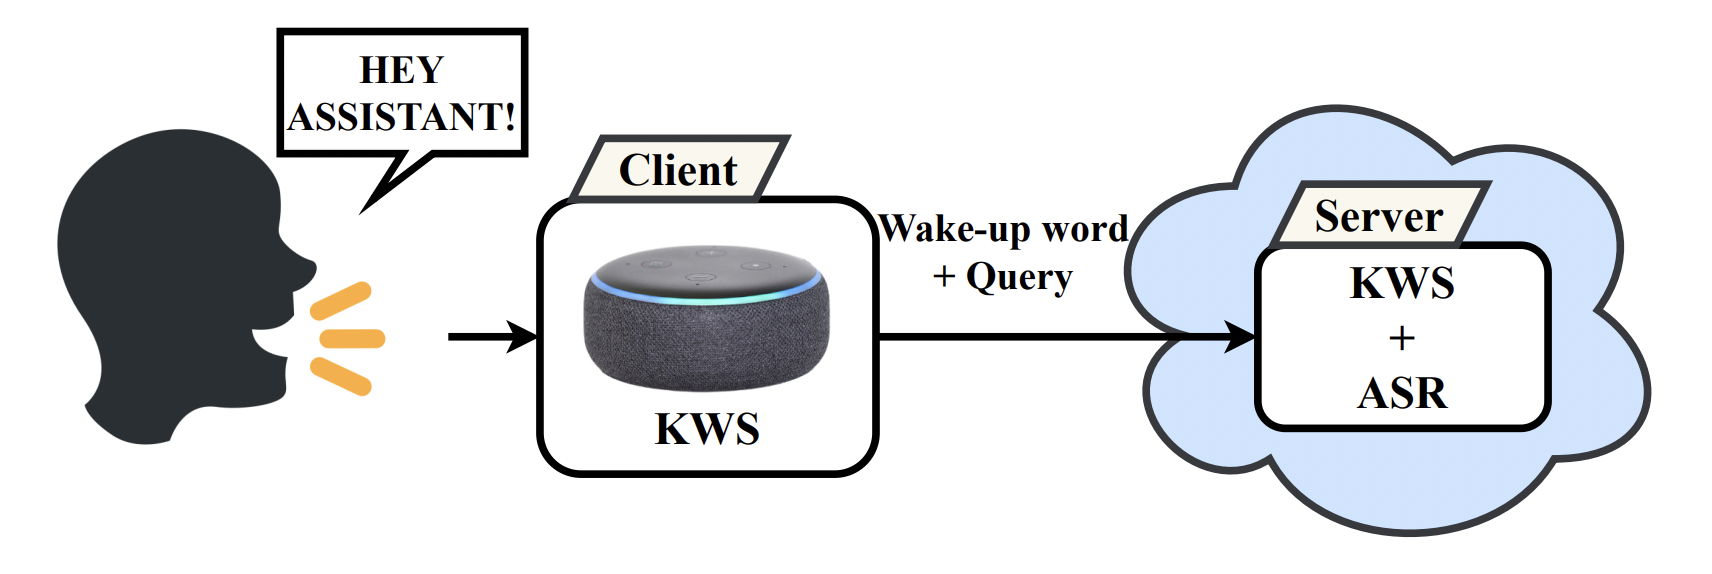
\includegraphics[width=0.99\linewidth]{figs/kws_pipeline.png}
    	\caption{Typical voice assistant client-server framework}
    \end{figure}
    What do we need? Lightweight robust ASR model
    
    \myfootnotewithlink{https://arxiv.org/pdf/2111.10592.pdf}{López-Espejo et al., Deep Spoken Keyword Spotting: An Overview, IEEE Access, 2021}

\end{frame}
%=======
\begin{frame}{KWS: quality}
    \begin{figure}
    	\centering
    	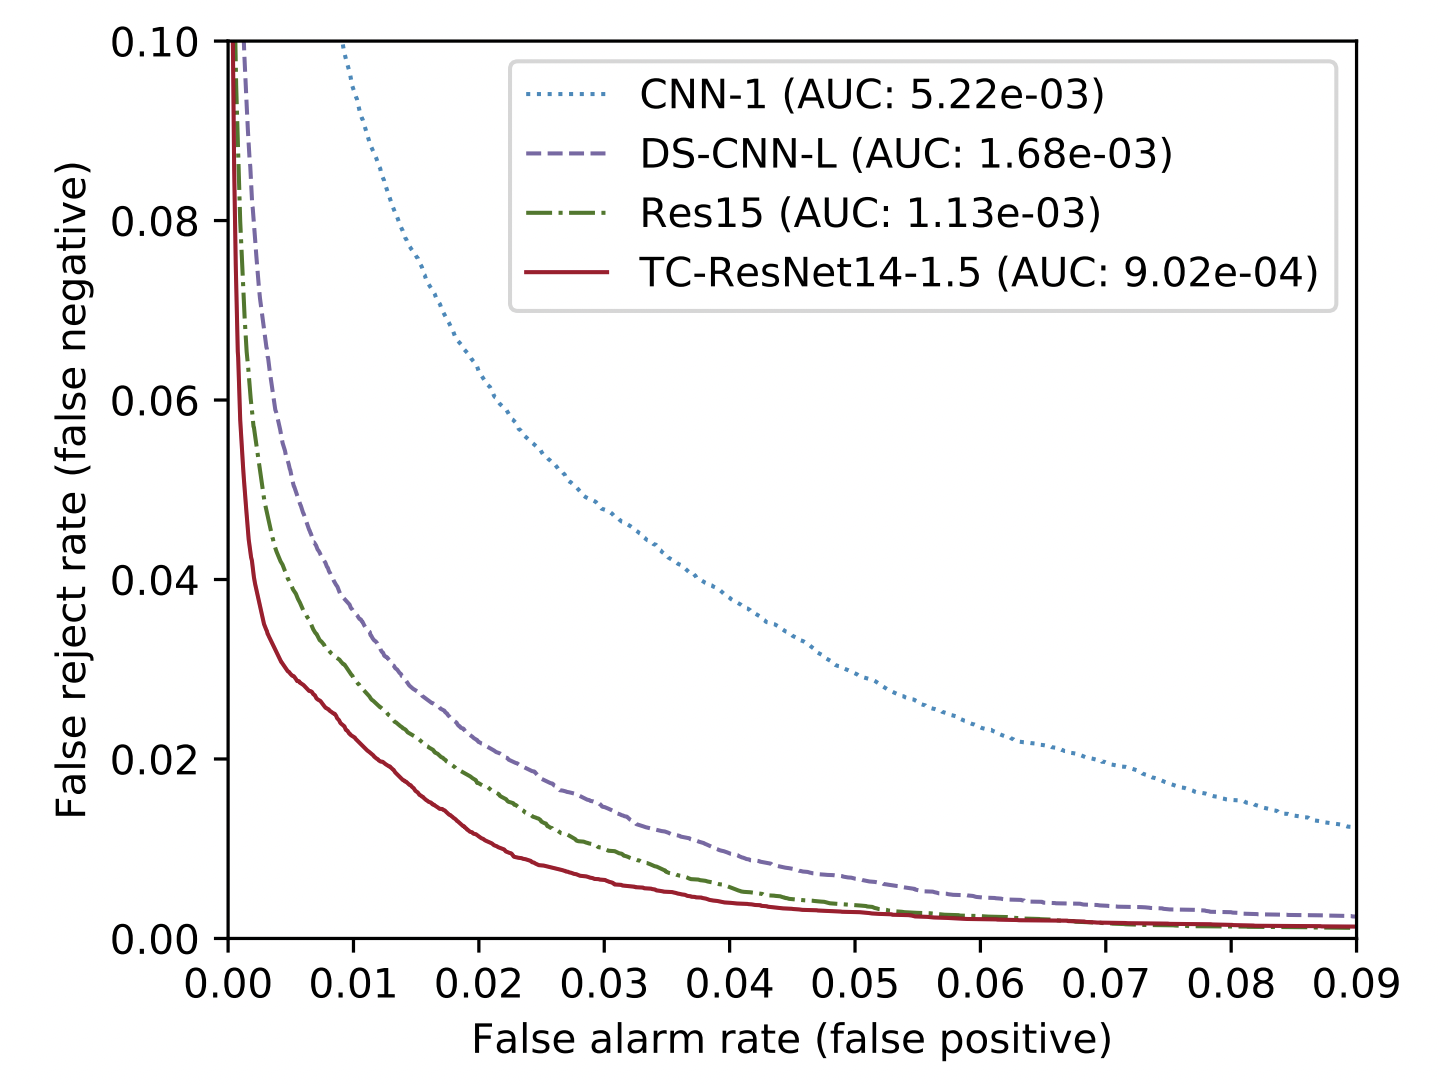
\includegraphics[width=0.65\linewidth]{figs/far_frr_plot.png}
    \end{figure}
    \begin{itemize}
        \item False alarm rate (false positive rate): $\mathrm{FAR}=\frac{\mathrm{FP}}{\mathrm{FP}+\mathrm{TN}}$
        \item False Reject Rate (false negative rate):
        $\mathrm{FNR}=\frac{\mathrm{FN}}{\mathrm{FN}+\mathrm{TP}}$
        \item FA/FR per hour, lower curves are better
    \end{itemize}
    
    \myfootnotewithlink{https://arxiv.org/pdf/1904.03814.pdf}{Choi et al., Temporal Convolution for Real-time Keyword Spotting on Mobile Devices, 2019}

\end{frame}
%=======
\begin{frame}{DNN based KWS}
    \begin{figure}
    	\centering
    	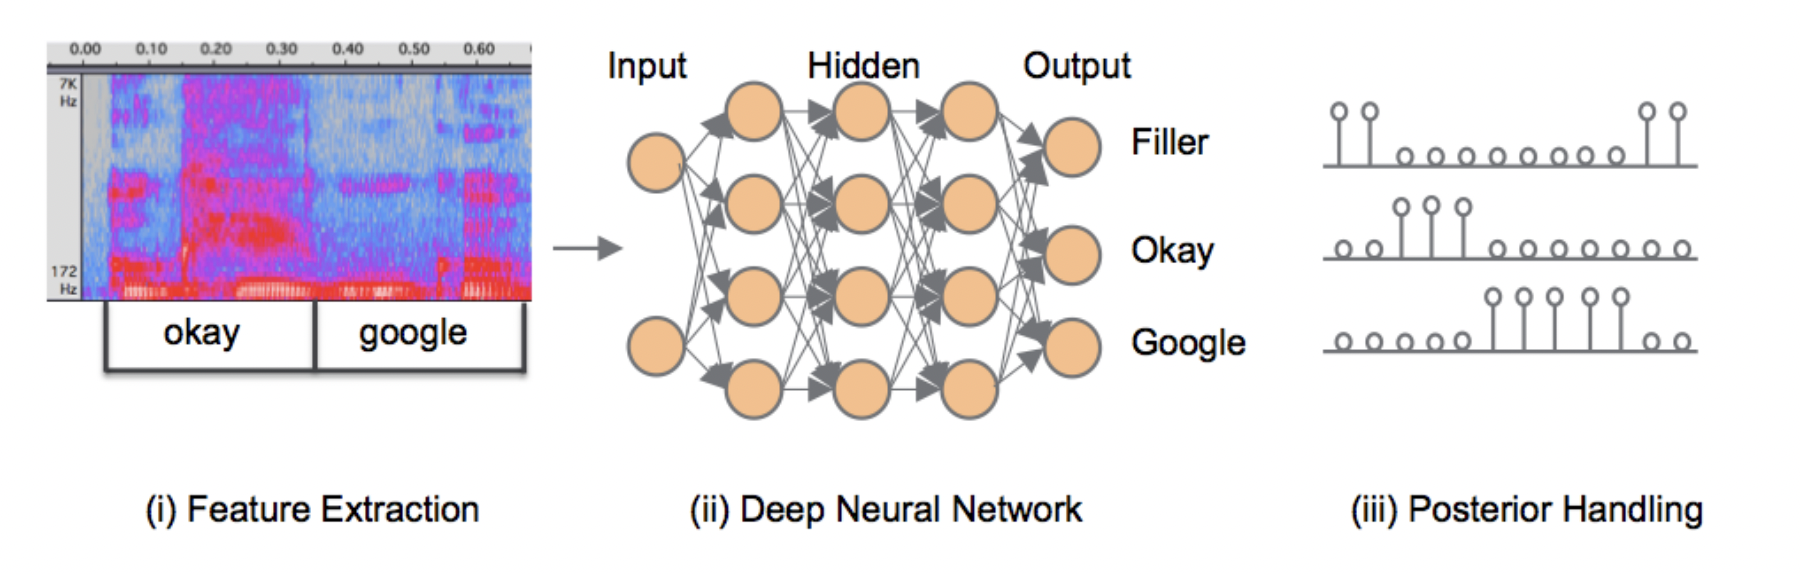
\includegraphics[width=0.9\linewidth]{figs/dnn_kws.png}
    \end{figure}
    \begin{itemize}
        \item Feature extraction: time windows $w_{smooth}$: 10 future frames + 30 frames in the past
        \item Raw posteriors from DNN are noisy, so smooth them over $w_{smooth}$
         $$p_{i j}^{\prime}=\frac{1}{j-h_{s m o o t h}+1}\sum_{k=h_{smooth}}p_{i j},$$
         $h_{smooth}=\operatorname*{max}\{\mathbf{1},j-w_{s m o o t h}+1\}$ -- the index of the first frame within the smoothing window
    \end{itemize}
    
    \myfootnotewithlink{https://static.googleusercontent.com/media/research.google.com/en//pubs/archive/42537.pdf}{Chen et al., Small-footprint keyword spotting using deep neural networks, IEEE International Conference on Acoustics, Speech and Signal Processing, 2014}

\end{frame}
%=======
\begin{frame}{CNN based KWS}
    \begin{figure}
    	\centering
    	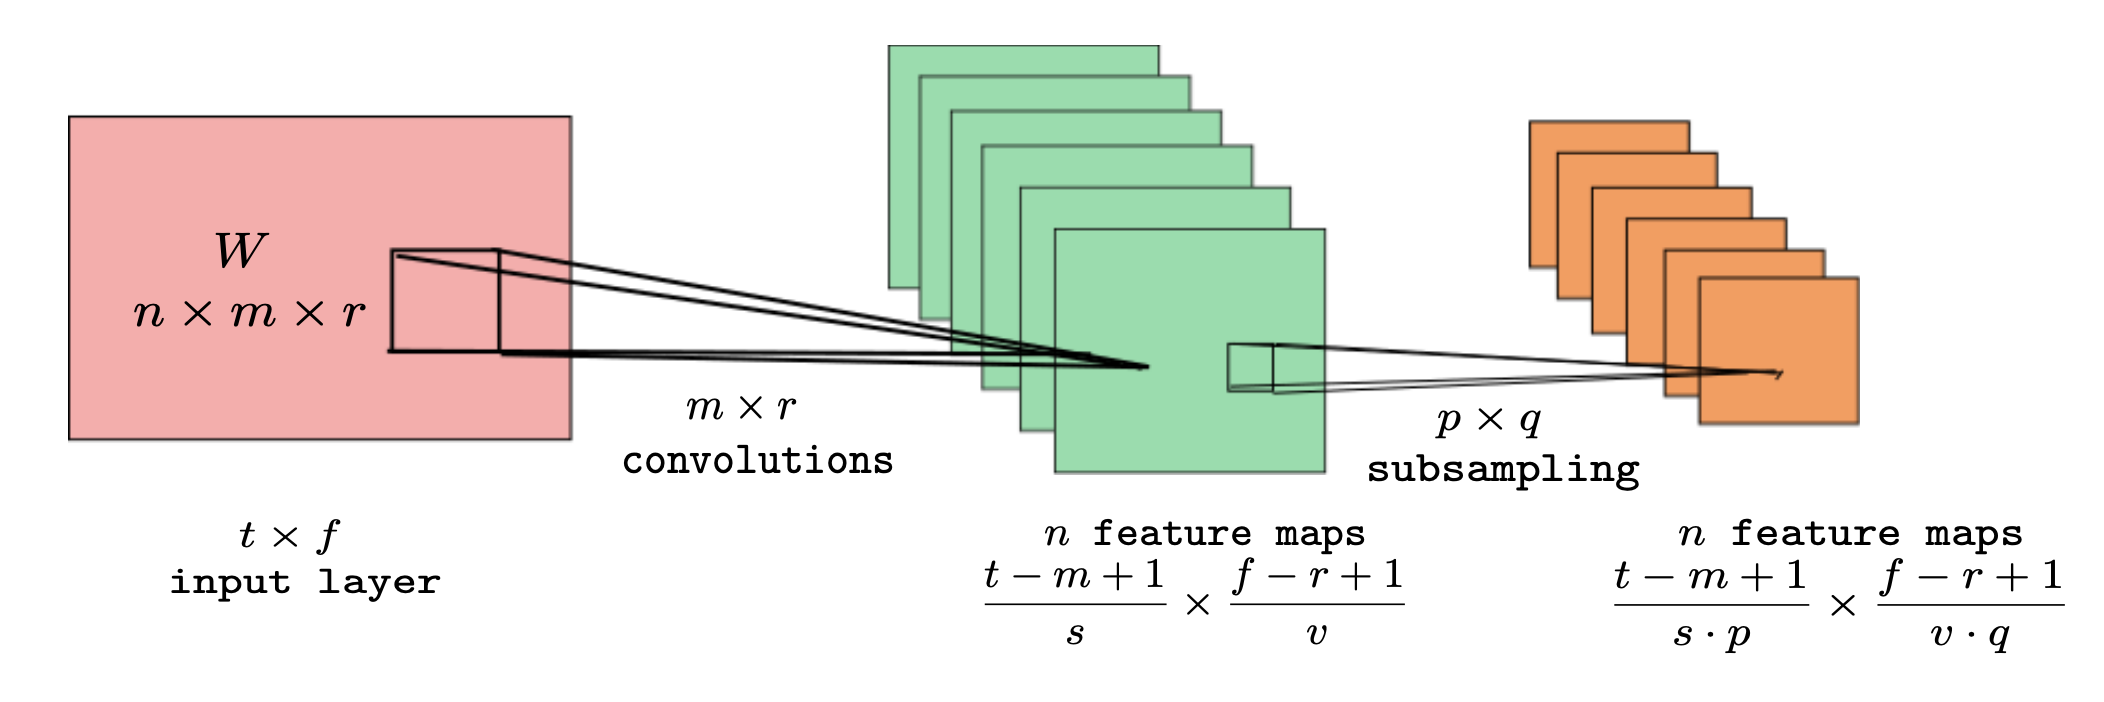
\includegraphics[width=0.99\linewidth]{figs/cnn_kws.png}
    	\caption{CNN architecture}
    \end{figure}
    
    \begin{itemize}
        \item Input signal $V \in \mathbb{R}^{t\times f}$, $t$ and $f$ -- input feature dimension in time and frequency. 
        \item Weight matrix $W \in \mathbb{R}^{(m\times r)\times n}$ is convolved with input $V$
        \item Filter of size $m\times r$, stride by $s$ in time and $v$ in frequency
        \item Pooling size $p \times q$
    \end{itemize}
    
    \myfootnotewithlink{https://static.googleusercontent.com/media/research.google.com/en//pubs/archive/43969.pdf}{Sainathet al., Convolutional neural networks for small-footprint keyword spotting, INTERSPEECH, 2015}

\end{frame}
\begin{frame}{Attention-based KWS}
    \begin{minipage}{0.55\textwidth}
        \begin{figure}
        	\centering
        	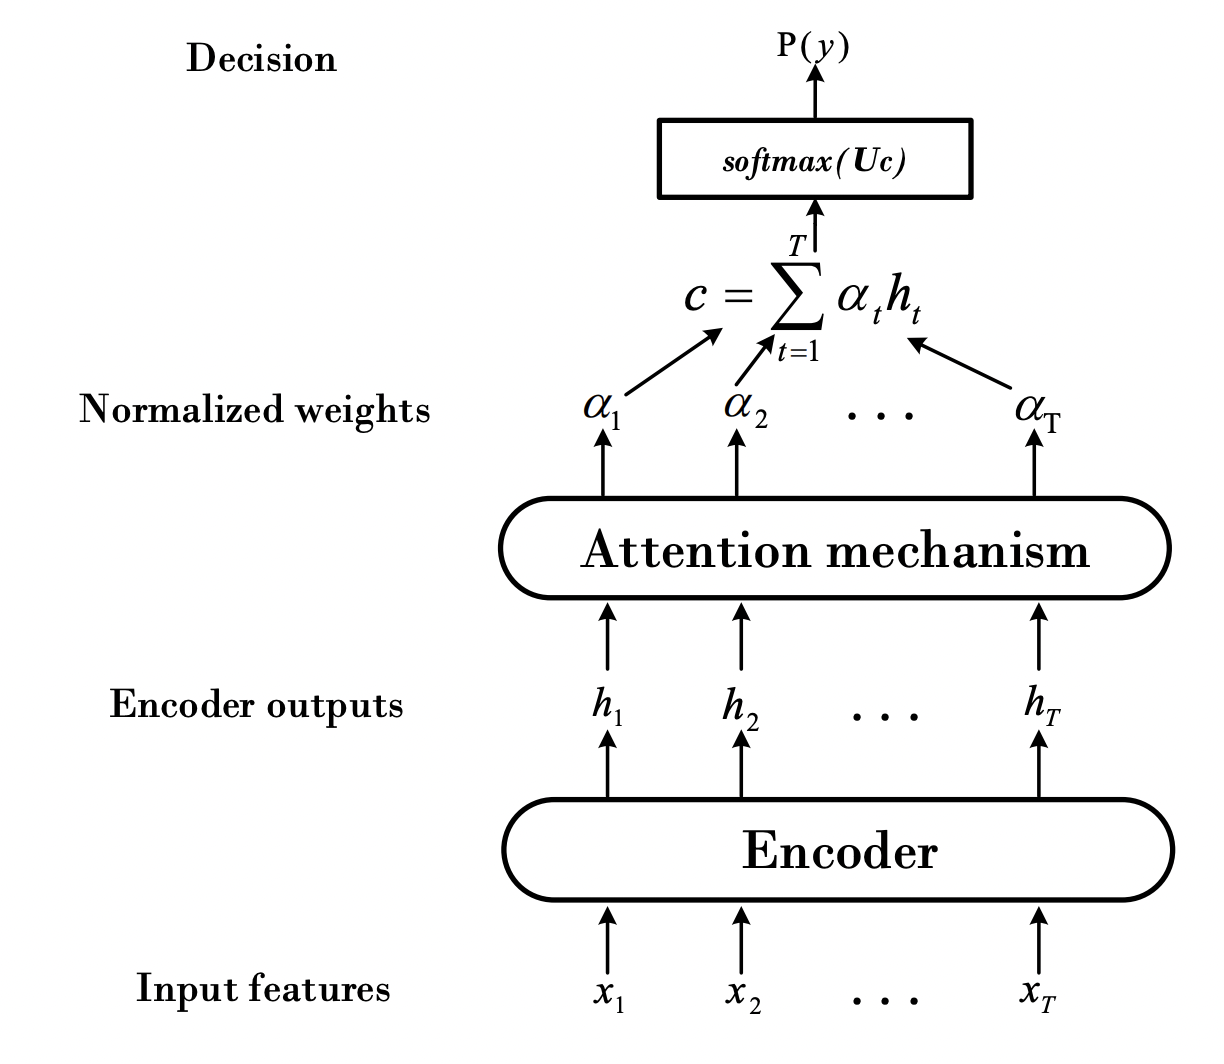
\includegraphics[width=0.95\linewidth]{figs/attention_kws.png}
        \end{figure}
    \end{minipage}%
    \hfill%
    \begin{minipage}{0.45\textwidth}
    \begin{itemize}
        \item Encoder: RNN/GRU/LSTM/CRNN
        ${\bf h}=Encoder({\bf x})$\\
        \item Soft attention: \\ 
        $e_{t}=v^{T}tanh(\bf W h_{t}+\bf b).$\\
        $\alpha_{t}=\frac{e x p(e_{t})}{\sum_{j=1}^{T}e x p(e_{j})}.$\\ \\
        $\bf c=\sum_{t=1}^{T}\alpha_{t}\bf h_{t}.$
    \end{itemize}
    \end{minipage}
    \myfootnotewithlink{https://arxiv.org/pdf/1803.10916.pdf}{Shan et al., Attention-based End-to-End Models for Small-Footprint Keyword Spotting, 2018}

\end{frame}
%=======
\begin{frame}{Multihead attention based KWS}
\begin{minipage}{0.5\textwidth}% adapt widths of minipages to your needs
    	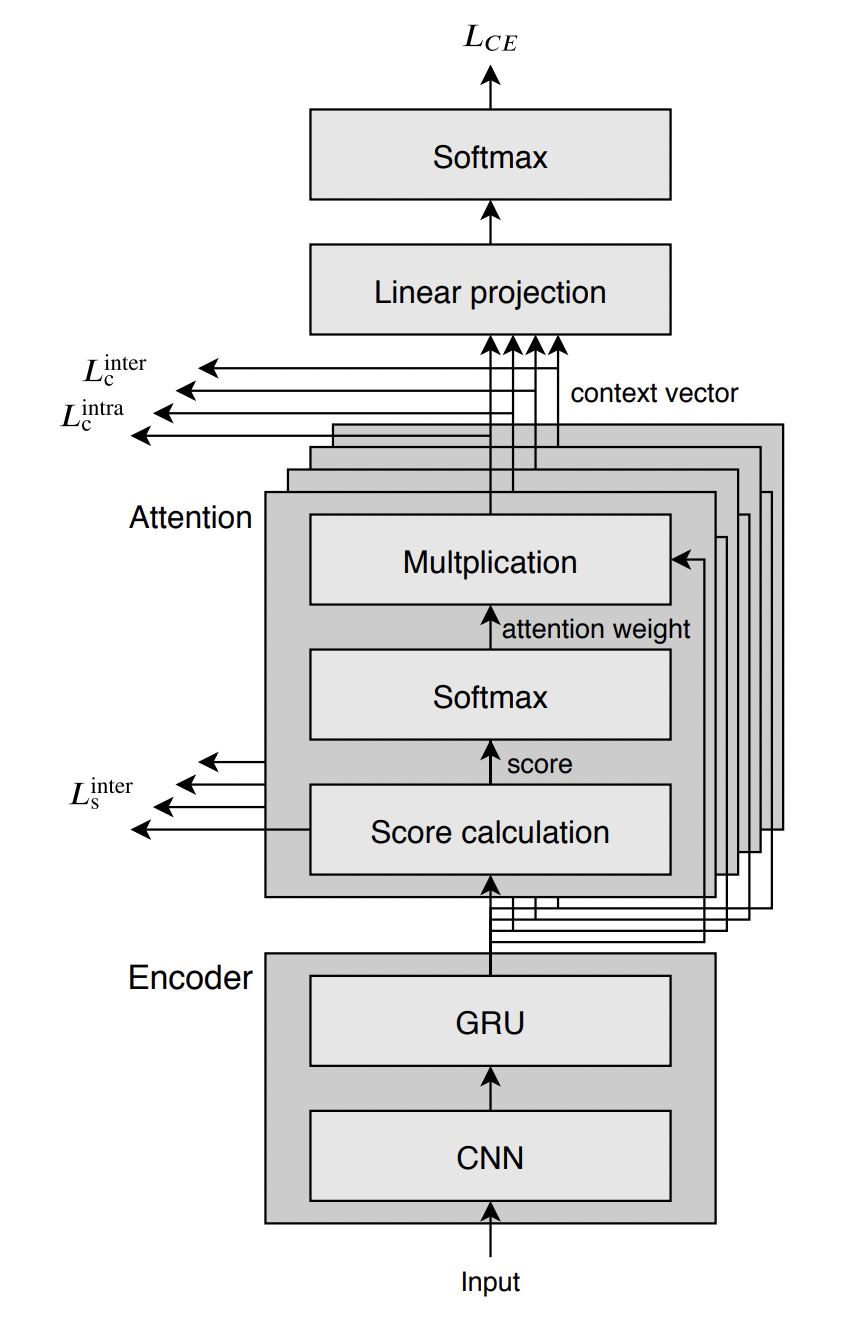
\includegraphics[width=0.9\linewidth]{figs/multihead_attention_kws.png}
\end{minipage}%
\hfill%
\begin{minipage}{0.5\textwidth}
\begin{itemize}
    \item Retrieves richer information than a single-head attention \\ 
    which only summarizes the whole sequence into one context vector
    \item The diversity is not guaranteed by its natural form $\rightarrow$ use Orthogonality regularization
\end{itemize}
\end{minipage}

    \myfootnotewithlink{https://arxiv.org/pdf/1803.10916.pdf}{Lee et al., Orthogonality Constrained Multi-Head Attention for Keyword Spotting, IEEE Automatic Speech Recognition and Understanding Workshop, 2019}


\end{frame}
%=======
\begin{frame}{Multihead attention based KWS: orthogonality}
    \begin{figure}
    	\centering
    	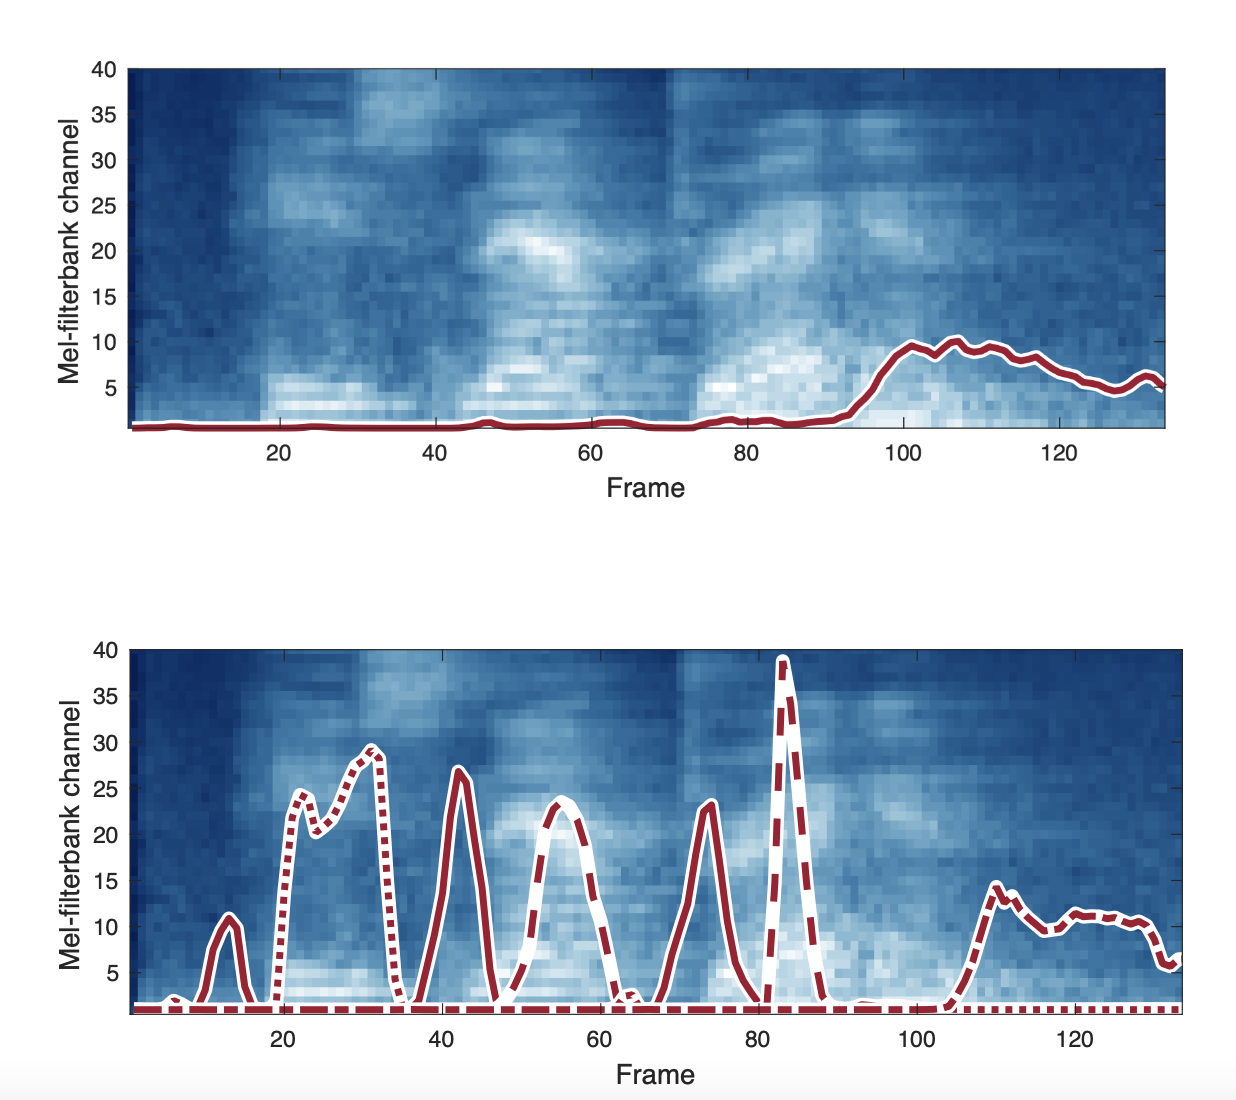
\includegraphics[width=0.7\linewidth]{figs/ortho_attention.png}
    	\caption{Attention weights overlaid on Mel-spectrogram with the configurations of single head attention (top), 4-head attention with regularization (bottom)}
    \end{figure}

\end{frame}
%=======
\begin{frame}{Multihead attention based KWS: orthogonality}
    \begin{itemize}
        \item Context matrix and the score matrix from normalized vectors (H -- number of attention heads):
        $${\bf C}^{(n)}=\left[{\overline{{{\bf c}}}}_{1}^{(n)},{\overline{{{{\bf c}}}}}_{2}^{(n)},\dots{\overline{{{{\bf c}}}}}_{H}^{(n)}\right],
        ~~~ \mathbf{E}^{(n)}\,=\,\left[\overline{{{\mathbf{e}}}}_{1}^{(n)},\overline{{{\mathbf{e}}}}_{2}^{(n)},\ldots\mathbf{\bf\overline{e}}_{H}^{(n)}\right]$$
    
        \item Inter-head orthogonality regularization
    $${{\mathcal{L}}_{\mathrm{c}}^{\mathrm{inter}}=\frac{1}{N_{\mathrm{P}}}\sum_{n=1}^{N}\frac{y^{(n)}}{H(H-1)}\left|\right|{\bf C}^{(n)\mathrm{T}}{\bf C}^{(n)}-{\bf I}_{H}\left|\right|_{F}^{2}}$$
    $${\mathcal{L}}_{s}^{\mathrm{inter}}=\frac{1}{N_{\bf P}}\sum_{n=1}^{N}\frac{y^{(n)}}{H(H-1)}\left|\right|{\bf E}^{(n)\mathrm{T}}{\bf E}^{(n)}-{\bf I}_{H}\left|\right|_{F}^{2}$$
    
    \item Intra-head non-orthogonality regularization
    $${\mathcal{L}}_{\mathrm{c}}^{\mathrm{intra}}={\frac{1}{H}}\sum_{i=1}^{H}{\frac{1}{N_{\mathrm{P}}(N_{\mathrm{P}}-1)}}\left\|\mathbf{Y}(\widetilde{\mathbf{C}}_{i}^{\mathrm{T}}\widetilde{\mathbf{C}}_{i}-\mathbf{I}_{N})\mathbf{Y}\right\|_{\mathrm{F}}^{2}$$
    
    \item Cross entropy loss with the regularization terms 
    $$\theta^{*}=\arg\operatorname*{min}\{\mathcal{L}_{\mathrm{CE}}+\lambda_{1}{\mathcal{L}}_{\mathrm{c}}^{\mathrm{inter}}-\lambda_{2}{\mathcal{L}}_{\mathrm{c}}^{\mathrm{intra}}+\lambda_{3}{\mathcal{L}}_{\mathrm{s}}^{\mathrm{inter}}\}$$
    \end{itemize}
    
\end{frame}
%=======
\begin{frame}{Single Value Decomposition Filter (SVDF)}
    \begin{figure}
    	\centering
    	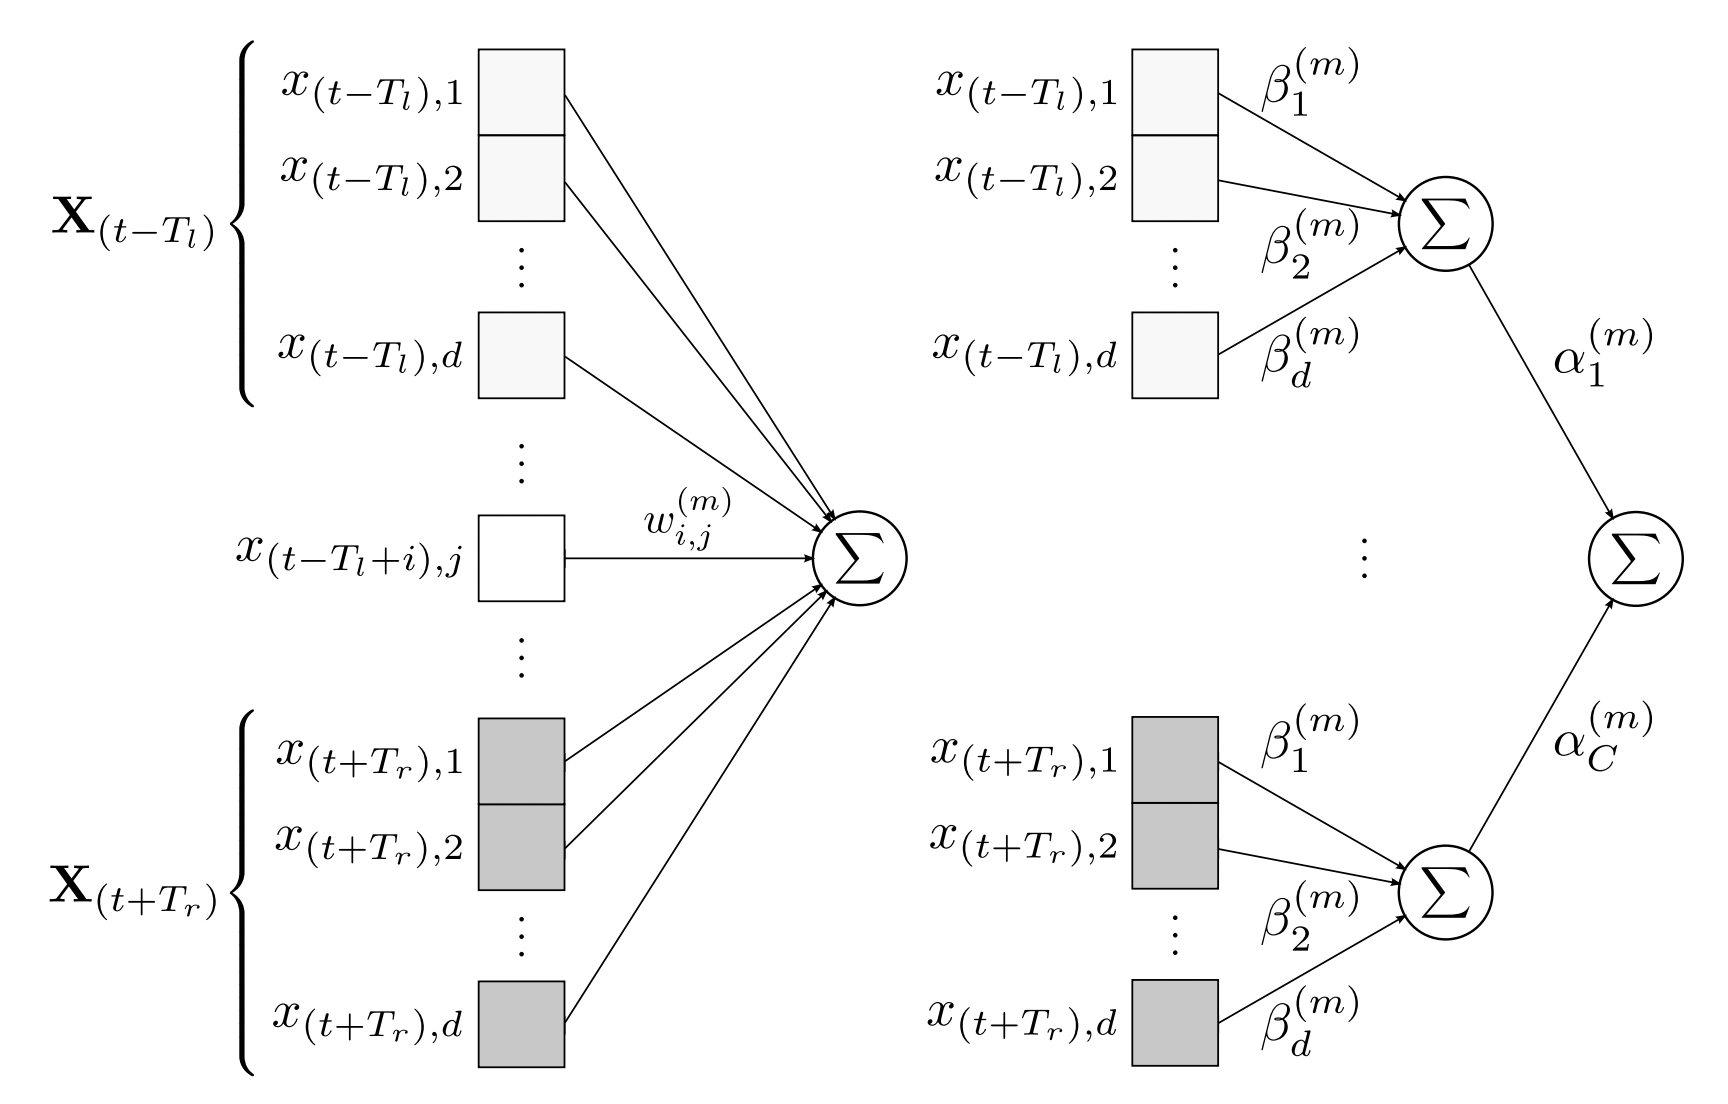
\includegraphics[width=0.65\linewidth]{figs/svdf_kws.png}
    \end{figure}

Before: 
$a_{t}^{(m)} = f\left(\sum_{i=0}^{C-1}\sum_{j=1}^{d}w_{i,j}^{(m)}x_{(t-T_{l}+i),j}\right)$\\
After:
$$a_{t}^{(m)}\approx f\left(\sum_{i=0}^{C-1}\alpha_{i}^{(m)}\sum_{j=1}^{d}\beta_{j}^{(m)}x_{(t-T_{l}+i),j}\right),~~~{w}_{i,j}^{\left(m\right)}\approx{\alpha}_{i}^{\left(m\right)}\beta_{j}^{\left(m\right)}$$

    \myfootnotewithlink{https://static.googleusercontent.com/media/research.google.com/en//pubs/archive/43813.pdf}{Nakkiran, Preetum et al., Compressing deep neural networks using a rank-constrained topology, INTERSPEECH 2015}

\end{frame}
%=======
\begin{frame}{Broadcasted Residual Learning}
    \begin{figure}
    	\centering
    	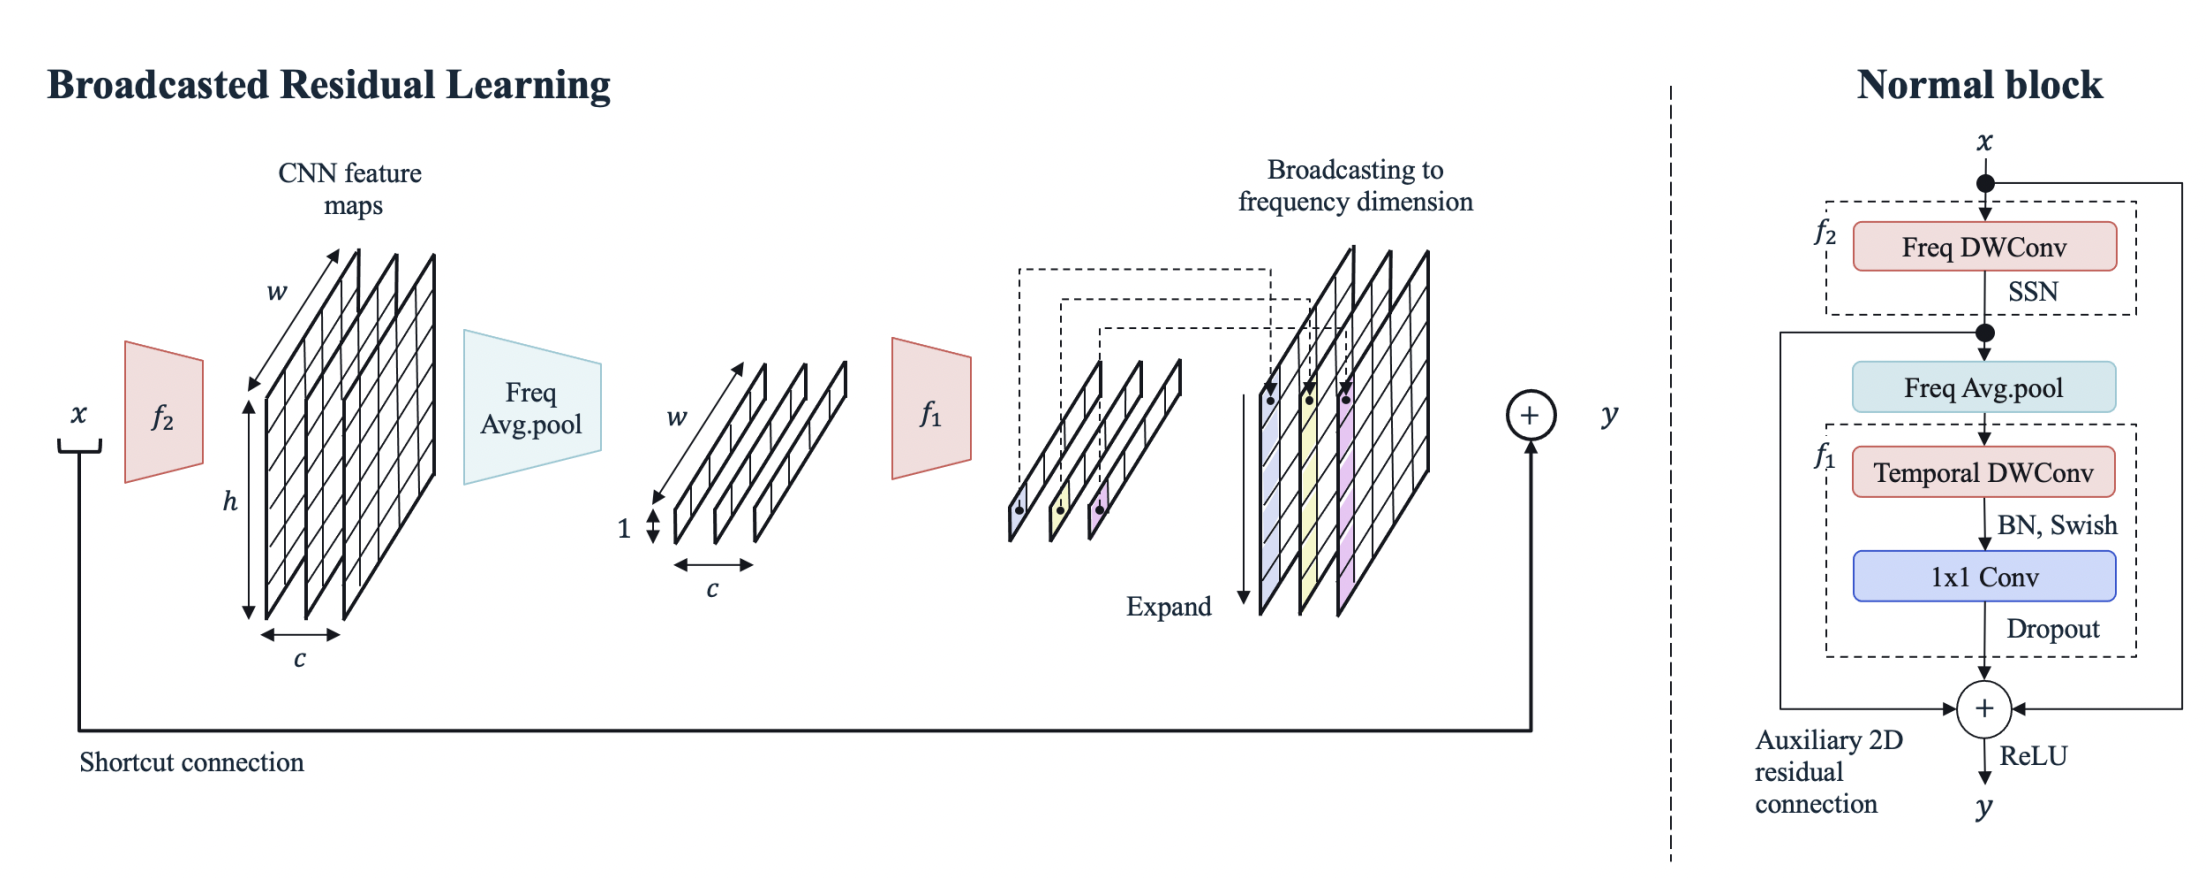
\includegraphics[width=0.99\linewidth]{figs/broadcasted_residual_kws.png}
    	\caption{\textbf{Left, Broadcasted Residual Learning} $y=x+B C(f_{1}(\avgpool(f_{2}(x))))$, number of channels $c$. \\ \textbf{Right, BCResBlock} $y=x+f_{2}(x)+B C(f_{1}(avgpool(f_{2}(x)))).$}
    \end{figure}
        
    \myfootnotewithlink{https://arxiv.org/pdf/2106.04140v2.pdf}{Kim, Byeonggeun et al., Broadcasted Residual Learning for Efficient Keyword Spotting., Interspeech, 2021}
    
\end{frame}
%=======
\begin{frame}{Convolutions in audio}
    \begin{figure}
    	\centering
    	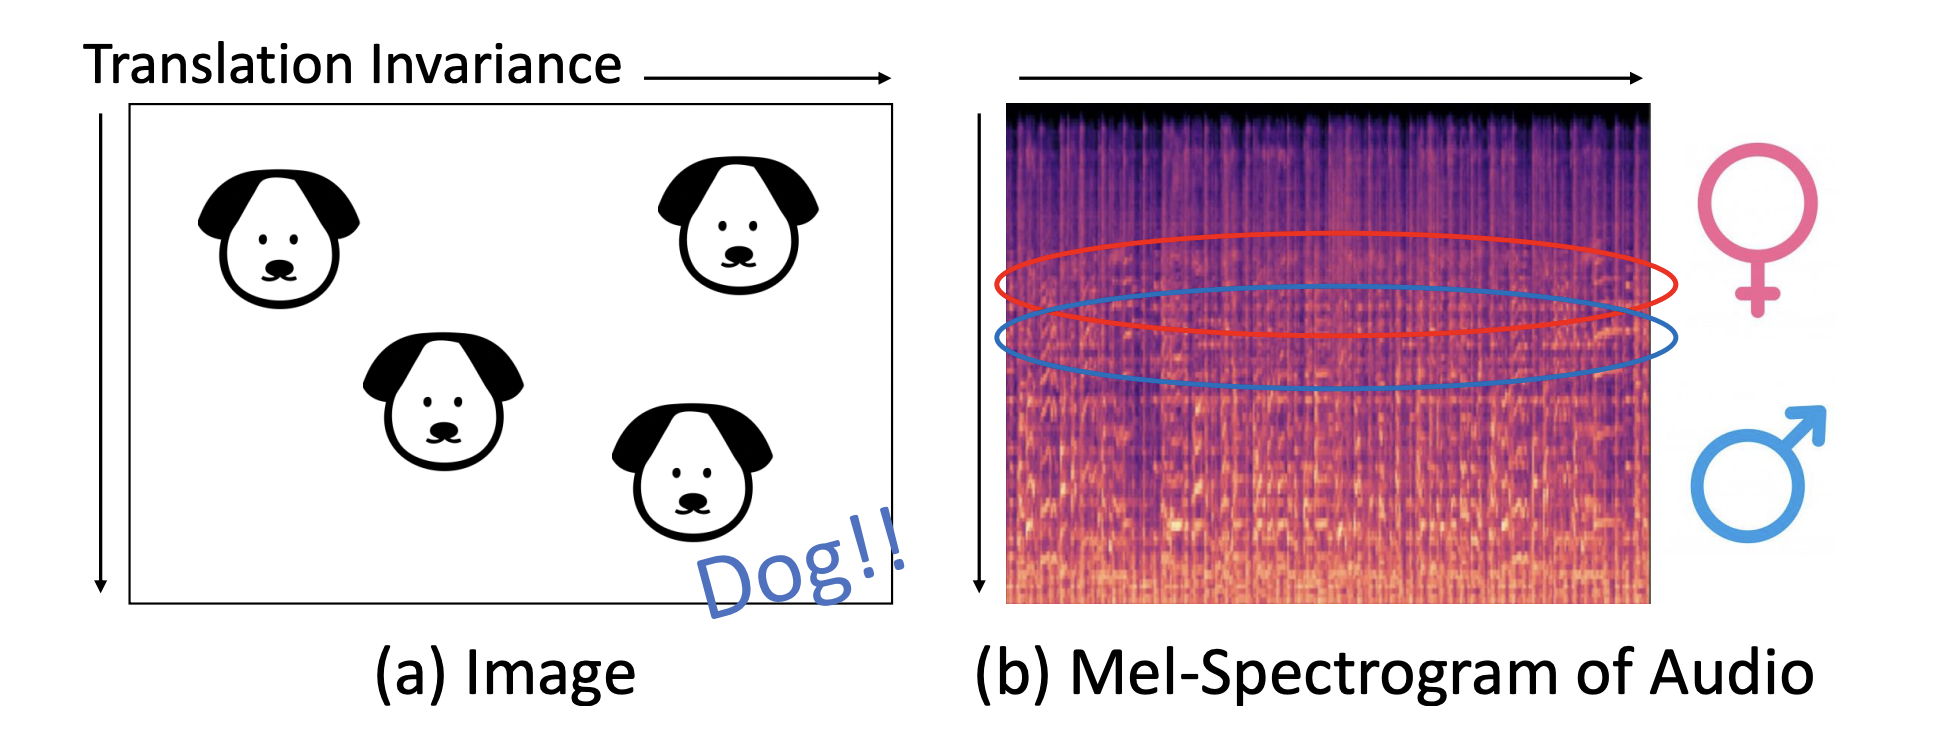
\includegraphics[width=0.99\linewidth]{figs/convolution_audio.png}
    	\caption{2D convolution on image and audio input: unlike image processing, the feature in different audio frequency bands has different information.}
    \end{figure}

\end{frame}
%=======
\begin{frame}{Subspectral Normalization (SSN)}
    \begin{figure}
    	\centering
    	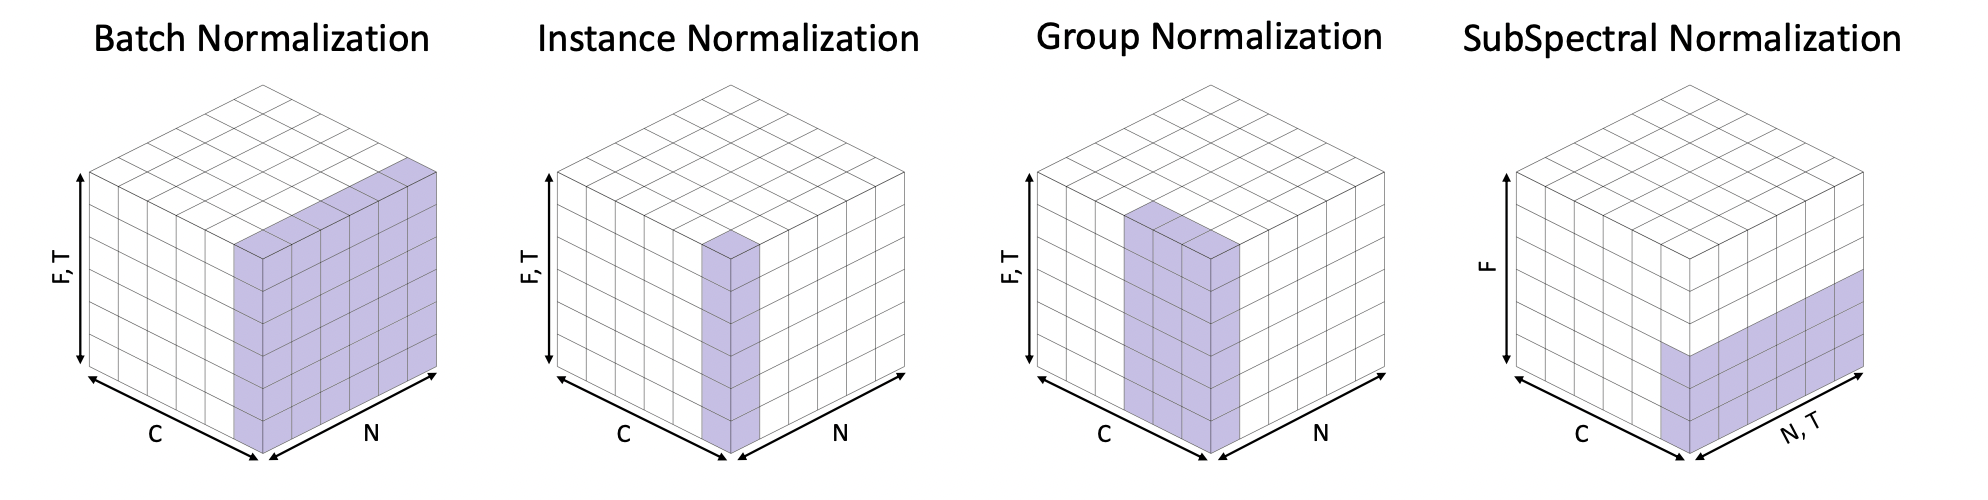
\includegraphics[width=0.99\linewidth]{figs/subspectral_normalization.png}
    	\caption{Normalization methods on Frequency-Time audio input, N -- batch axis, C -- channels, F -- frequency, T -- time axis. SSN splits the frequency dimension into multiple sub-bands and normalizes each group}
    \end{figure}
    
    \myfootnotewithlink{https://arxiv.org/pdf/2103.13620.pdf}{Chang et al., SubSpectral Normalization for Neural Audio Data Processing, 2021}
\end{frame}
%=======
\begin{frame}{Keyword Transformer based KWS}
    \begin{figure}
    	\centering
    	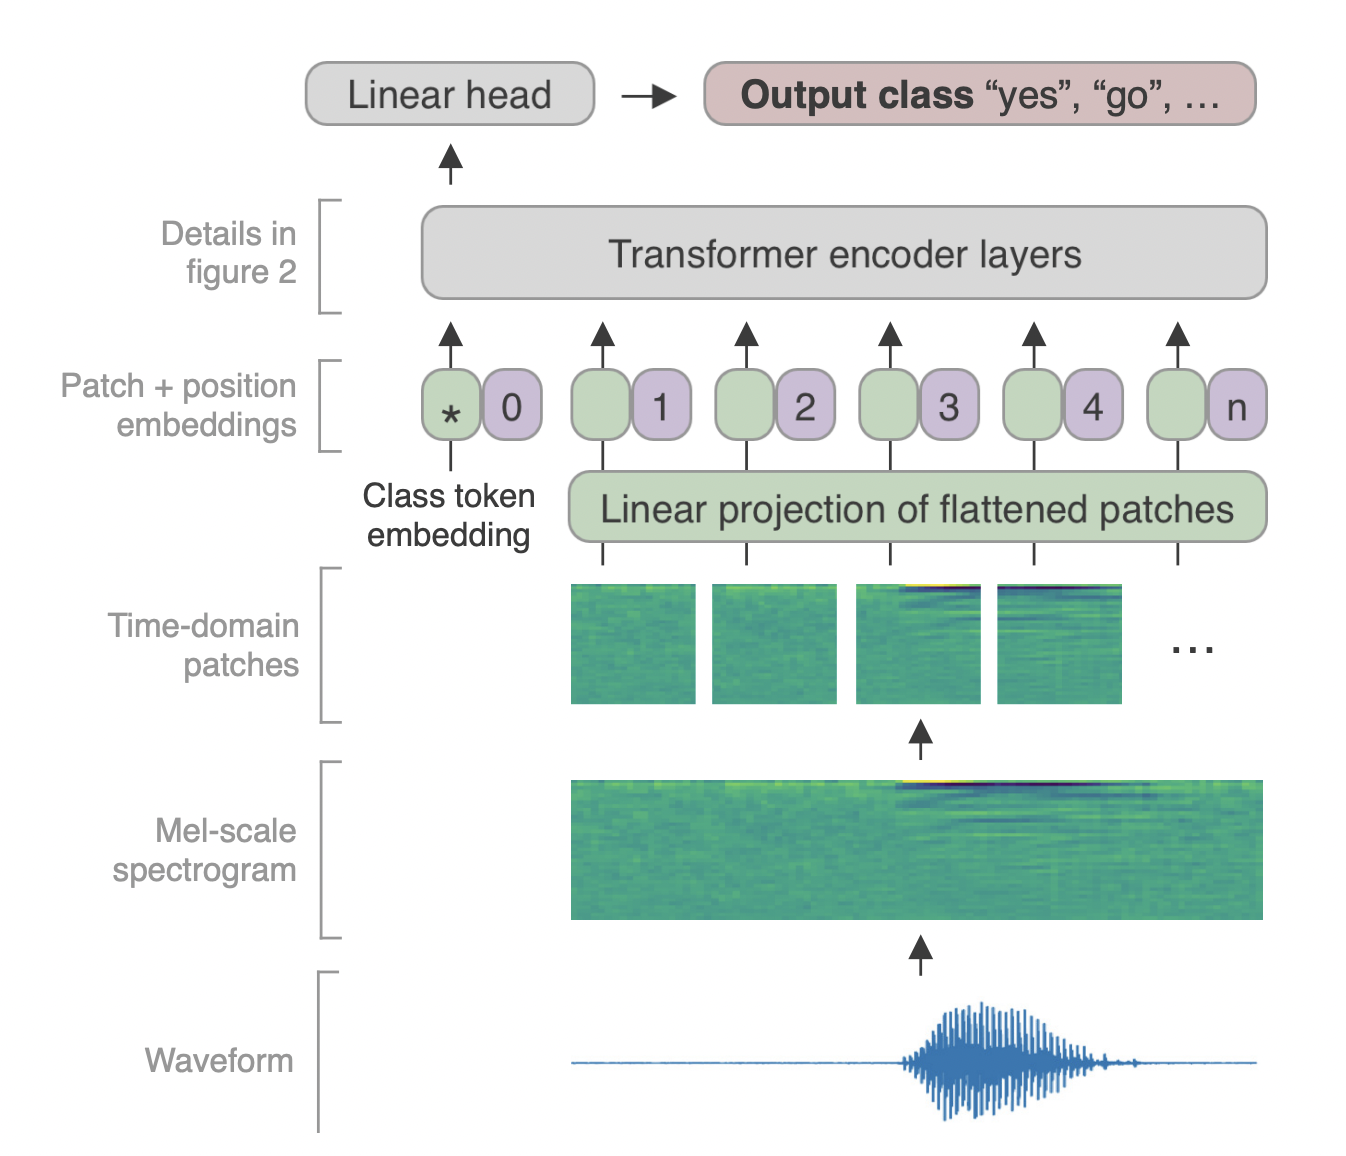
\includegraphics[width=0.7\linewidth]{figs/transformer_kws.png}
    	\caption{Keyword Transformer architecture}
    \end{figure}
    
    \myfootnotewithlink{https://arxiv.org/pdf/2104.00769.pdf}{Berg et al., Keyword Transformer: A Self-Attention Model for Keyword Spotting. Interspeech, 2021}
\end{frame}
%=======
\begin{frame}{KWS: summary}

\begin{table}[]
\begin{tabular}{|c|c|c|c|}
\hline
\textbf{KWS Idea}                                                               & \textbf{Year/Company}                                                   & \textbf{Params} & \textbf{\begin{tabular}[c]{@{}c@{}}Accuracy,\\ V1 dataset\end{tabular}} \\ \hline
DNN                                                                             & 2014, Google                                                            & $\sim$224k      & 91.2                                                                    \\ \hline
CNN                                                                             & 2015, Google                                                            & 20-70k          & 95.4                                                                    \\ \hline
Attention                                                                       & 2018, Xiaomi                                                            & $\sim$84k       & 95.6                                                                    \\ \hline
\begin{tabular}[c]{@{}c@{}}Multihead\\ attention\end{tabular}                   & 2019, Qualcomm                                                          & 743k               & 97.2                                                                    \\ \hline
\begin{tabular}[c]{@{}c@{}}Single Value \\ Decomposition \\ Filter\end{tabular} & \begin{tabular}[c]{@{}c@{}}2015/2019, \\ Google\end{tabular}            & 40-700k         & 96.3                                                                    \\ \hline
\begin{tabular}[c]{@{}c@{}}Broadcasted \\ Residual\end{tabular}                 & 2021,  Qualcomm                                                         & 9.2k            & 96.6                                                                    \\ \hline
\begin{tabular}[c]{@{}c@{}}Subspectral \\ Normalization\end{tabular}            & 2021, Qualcomm                                                          & 113-243k        & 97.5                                                                    \\ \hline
Transformer                                                                     & \begin{tabular}[c]{@{}c@{}}2021, \\ Arm ML \\ Research Lab\end{tabular} & 607-5361k*      & 97.5                                                                    \\ \hline
\end{tabular}
\end{table}
%https://arxiv.org/pdf/2005.06720v2.pdf
\end{frame}
%=======
\section{KWS problems and practices}
%=======
\begin{frame}{Class imbalance}
\begin{itemize}
    \item Oversampling 
    \begin{figure}
    	\centering
    	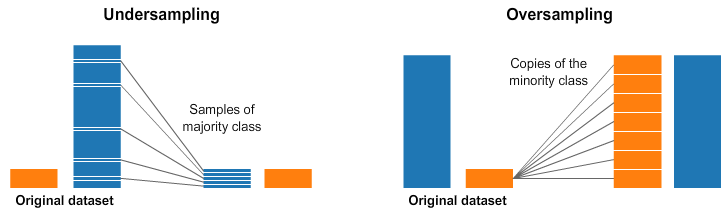
\includegraphics[width=0.65\linewidth]{figs/oversampling_imbalance.png}
    \end{figure}
    \item Class weighted Cross-entropy (CE)
    \item Focal Loss
    \begin{figure}
    	\centering
    	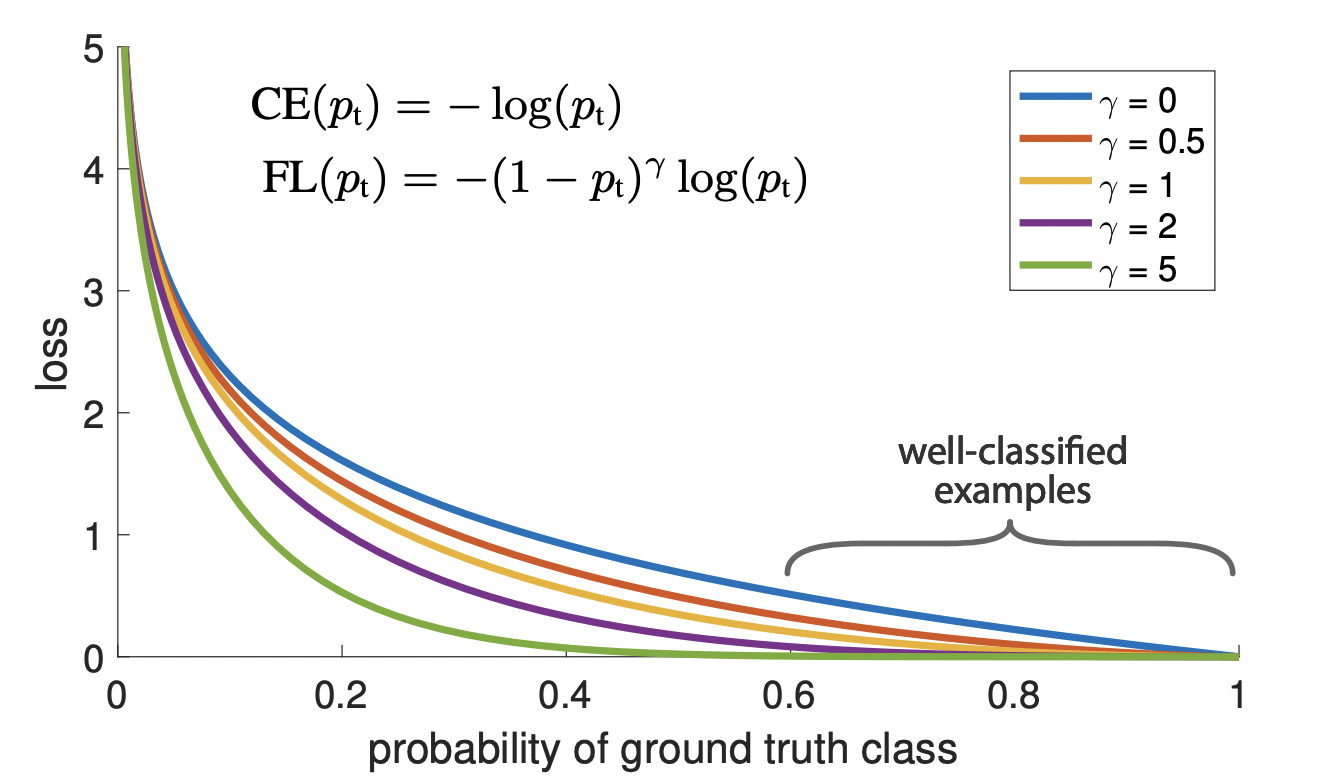
\includegraphics[width=0.65\linewidth]{figs/focal_loss.png}
    \end{figure}
\end{itemize}

    \myfootnotewithlink{https://arxiv.org/pdf/1708.02002.pdf}{Lin, Goyal et al., Focal Loss for Dense Object Detection, in IEEE Transactions on Pattern Analysis and Machine Intelligence, vol. 42, 2020}

\end{frame}
%=======
\begin{frame}{Robustness}
\begin{itemize}
    \item Multitask learning: Train ASR and KWS simultaneously
    $$\mathcal{L}=\gamma\mathcal{L}^{(1)}+(1-\gamma)\mathcal{L}^{(2)},\;\;\;\;\;\;0\leq\gamma\underline{{{<1}}}$$
    \item Augmentations
    \begin{itemize}
        \item Pitch and Tempo
        \item Time shifts
        \item Resampling
        \item Environment Simulation
        \item Background noise
    \end{itemize}
    \item Hard negative mining
    \item Federated Learning
    \item Clean data
\end{itemize}
\end{frame}
%=======

\end{document} 
